\chapter{Результаты работы}
\section{Архитектура системы}
Архитектура системы представляет собой модульную систему. Основными компонентами системы являются:
\begin{enumerate}
	\item TU webservice
	\item CoreService
	\item DataService
	\item Reasoner
	\item ClientAgent
	\item MessageBus
\end{enumerate}
Система может работать в 2-х режимах: режим обучения и режим запроса. Вариант использования для режима обучения представлен на Рисунке \ref{img:train}. Главными действующими лицами является специалист технической поддержки (TSS), в общем случае это базовый класс Пользователь (User). Данный вариант использования имеет несколько ветвей:
\begin{itemize}
	\item communication:Train - обучение посредством коммуникации с системой специалиста технической поддержки. 
	\item communication:ProvidesSolution - в случае коммуникации в режиме обучения специалист технической поддержки должен предоставить не только сам запрос, который будет формализован системой, но также решение данного запроса. Система формализует запрос, формализует решение и создаст между ними связи
	\item communication:ProvideRequest - специалист технической поддержки вводит в систему запрос
	\item communication:MonitorsSolution - специалист технической поддержки смотрит как применяется решение, если находится проблема, то решение корректируется в CorrectSystemSolutions
\end{itemize}
\begin{figure} [h] 
  \center
  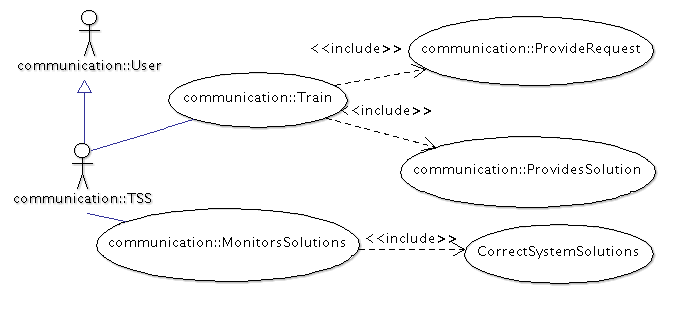
\includegraphics [scale=1.0] {UseCaseTrain}
  \caption{K-line} 
  \label{img:train}  
\end{figure}
Второй вариант использования это основной кейс. Главными действующими лицами системы является заказчик (Customer), в общем случае это базовый класс Пользователь (User). Он также имеет несколько ветвей:
\begin{itemize}
	\item ProvideRequest - заказчик вводит запрос в систему. Это может быть либо команда ProvideDirectInstruction, либо описание проблемы ProvideProblemDescription.
	\item communication:ProvideClarificationResponse - в случае, если система не может формализовать запрос, либо нашлось множество решений, то система запрашивает пользователя детали
	\item communication:ProvideConfirmationResponse - в случае, когда система нашла решение, она запрашивает пользователя подтверждение о том, что искомое решение решило его проблему
\end{itemize}
\section{Прототип}
\section{Испытание прототипа}
\section{Выводы по главе}
%\newpage
%============================================================================================================================


\clearpage